\documentclass[aspectratio=169,11pt]{beamer}

% Theme and colors
\usetheme{Madrid}
\usecolortheme{whale}
\setbeamertemplate{navigation symbols}{}
\setbeamertemplate{footline}[frame number]

% Packages
\usepackage[utf8]{inputenc}
\usepackage[T1]{fontenc}
\usepackage{graphicx}
\usepackage{booktabs}
\usepackage{amsmath}
\usepackage{hyperref}
\usepackage{tikz}
\usetikzlibrary{shapes,arrows,positioning,calc,fit,backgrounds,decorations.pathmorphing,patterns}
\usepackage{siunitx}

% Custom colors
\definecolor{questionbg}{RGB}{255,248,220}
\definecolor{questionborder}{RGB}{255,193,7}

% Title information
\title[EECE5155 -- Module 5]{The Network Layer}
\subtitle{Module 5: Routing, Addressing, and IoT Networking}
\author{Eduardo Baena}
\date{Spring 2026}
\institute{Northeastern University\\Department of Electrical and Computer Engineering\\
\texttt{e.baena@northeastern.edu}}

\begin{document}

% Title slide
\begin{frame}
    \titlepage
    \vspace{-1cm}
    \begin{center}
        \textbf{EECE5155: Wireless Sensor Networks and the Internet of Things}
    \end{center}
\end{frame}

% Learning Objectives
\begin{frame}{Learning Objectives}
    \textbf{By the end of this module, you should be able to:}
    
    \vspace{0.5cm}
    \begin{enumerate}
        \item \textbf{Explain} the role of the network layer in end-to-end communication
        \item \textbf{Compare} routing algorithms (DVR, LSR, flooding) and their tradeoffs
        \item \textbf{Analyze} ad-hoc routing protocols (AODV, OLSR) for IoT scenarios
        \item \textbf{Apply} RPL concepts for Low-Power and Lossy Networks
        \item \textbf{Justify} IPv6 and 6LoWPAN adoption for IoT applications
    \end{enumerate}
    
    \vspace{0.3cm}
    \begin{alertblock}{Design Implication}
        Routing decisions directly impact \textbf{energy consumption}, \textbf{latency}, and \textbf{network lifetime} in battery-powered IoT deployments.
    \end{alertblock}
\end{frame}

% Outline
\begin{frame}{Outline}
    \tableofcontents
\end{frame}

%==============================================================================
\section{Network Layer Fundamentals}
%==============================================================================

\begin{frame}{The Protocol Stack}
    \begin{center}
    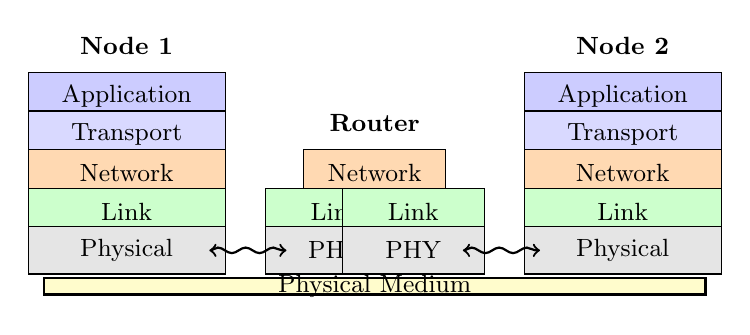
\begin{tikzpicture}[scale=0.7, every node/.style={font=\small}]
        % Node 1
        \node[draw, fill=blue!20, minimum width=2.5cm, minimum height=0.6cm] (app1) at (0,4) {Application};
        \node[draw, fill=blue!15, minimum width=2.5cm, minimum height=0.6cm] (trans1) at (0,3.3) {Transport};
        \node[draw, fill=orange!30, minimum width=2.5cm, minimum height=0.6cm] (net1) at (0,2.6) {Network};
        \node[draw, fill=green!20, minimum width=2.5cm, minimum height=0.6cm] (link1) at (0,1.9) {Link};
        \node[draw, fill=gray!20, minimum width=2.5cm, minimum height=0.6cm] (phy1) at (0,1.2) {Physical};
        \node[above=0.1cm of app1] {\textbf{Node 1}};
        
        % Intermediate nodes
        \node[draw, fill=orange!30, minimum width=1.8cm, minimum height=0.6cm] (net2) at (4.5,2.6) {Network};
        \node[draw, fill=green!20, minimum width=1.8cm, minimum height=0.6cm] (link2a) at (3.8,1.9) {Link};
        \node[draw, fill=green!20, minimum width=1.8cm, minimum height=0.6cm] (link2b) at (5.2,1.9) {Link};
        \node[draw, fill=gray!20, minimum width=1.8cm, minimum height=0.6cm] (phy2a) at (3.8,1.2) {PHY};
        \node[draw, fill=gray!20, minimum width=1.8cm, minimum height=0.6cm] (phy2b) at (5.2,1.2) {PHY};
        \node[above=0.1cm of net2] {\textbf{Router}};
        
        % Node 2
        \node[draw, fill=blue!20, minimum width=2.5cm, minimum height=0.6cm] (app2) at (9,4) {Application};
        \node[draw, fill=blue!15, minimum width=2.5cm, minimum height=0.6cm] (trans2) at (9,3.3) {Transport};
        \node[draw, fill=orange!30, minimum width=2.5cm, minimum height=0.6cm] (net3) at (9,2.6) {Network};
        \node[draw, fill=green!20, minimum width=2.5cm, minimum height=0.6cm] (link3) at (9,1.9) {Link};
        \node[draw, fill=gray!20, minimum width=2.5cm, minimum height=0.6cm] (phy3) at (9,1.2) {Physical};
        \node[above=0.1cm of app2] {\textbf{Node 2}};
        
        % Connections
        \draw[<->, thick, decorate, decoration={snake, amplitude=1pt}] (1.5,1.2) -- (2.9,1.2);
        \draw[<->, thick, decorate, decoration={snake, amplitude=1pt}] (6.1,1.2) -- (7.5,1.2);
        
        % Physical medium
        \draw[thick, fill=yellow!20] (-1.5,0.4) rectangle (10.5,0.7);
        \node at (4.5,0.55) {Physical Medium};
    \end{tikzpicture}
    \end{center}
    
    \vspace{0.3cm}
    \begin{alertblock}{Key Insight}
        The \textbf{Network Layer} enables end-to-end packet delivery across \textbf{multiple hops} and \textbf{heterogeneous networks}.
    \end{alertblock}
\end{frame}

\begin{frame}{Network Layer Objective}
    \textbf{Goal:} Enable end-to-end transmission between any source and destination nodes, even if they are \textbf{not on the same link or network}.
    
    \vspace{0.5cm}
    \textbf{Core Functionalities:}
    \begin{columns}
        \column{0.5\textwidth}
        \begin{block}{Routing}
            Find the \textbf{best paths} from source to destination considering network topology
        \end{block}
        
        \begin{block}{Internetworking}
            Enable interconnection of \textbf{different networks} regardless of underlying technology
        \end{block}
        
        \column{0.5\textwidth}
        \begin{block}{Load Balancing}
            Prevent congestion by \textbf{distributing traffic} across the network
        \end{block}
        
        \begin{block}{Addressing}
            Provide \textbf{logical addresses} independent of physical hardware
        \end{block}
    \end{columns}
\end{frame}

\begin{frame}{Routing Algorithm Properties}
    \textbf{Desired properties of routing algorithms:}
    
    \vspace{0.3cm}
    \begin{columns}
        \column{0.5\textwidth}
        \begin{itemize}
            \item \textbf{Correctness} -- packets reach destination
            \item \textbf{Simplicity} -- easy to implement
            \item \textbf{Robustness} -- handles failures gracefully
            \item \textbf{Stability} -- paths converge quickly
        \end{itemize}
        
        \column{0.5\textwidth}
        \begin{itemize}
            \item \textbf{Fairness} -- equitable resource allocation
            \item \textbf{Energy Efficiency} -- critical for IoT!
            \item \textbf{Scalability} -- works with many nodes
            \item \textbf{Low overhead} -- minimal control traffic
        \end{itemize}
    \end{columns}
    
    \vspace{0.5cm}
    \begin{alertblock}{IoT-Specific Consideration}
        Traditional routing optimizes for \textbf{delay} or \textbf{throughput}. IoT routing must also consider \textbf{energy consumption} and \textbf{node lifetime}.
    \end{alertblock}
\end{frame}

\begin{frame}{IoT vs Traditional Networks}
    \begin{columns}
        \column{0.5\textwidth}
        \textbf{Traditional Networks:}
        \begin{itemize}
            \item End nodes and routers are \textbf{different devices}
            \item End nodes: generate/receive data
            \item Routers: forward data between nodes
            \item Routers have dedicated power/resources
        \end{itemize}
        
        \column{0.5\textwidth}
        \textbf{Internet of Things:}
        \begin{itemize}
            \item Things act as \textbf{both} end nodes AND routers
            \item Often directly connected to gateway
            \item Multi-hop needed for coverage extension
            \item \textbf{Battery-powered} routing nodes!
        \end{itemize}
    \end{columns}
    
    \vspace{0.5cm}
    \begin{exampleblock}{Design Implication}
        When an IoT device acts as a router, it consumes energy forwarding \textbf{other nodes' traffic}. This affects network lifetime planning.
    \end{exampleblock}
\end{frame}

%==============================================================================
\section{Routing Algorithms}
%==============================================================================

\begin{frame}{Static vs Dynamic Routing}
    \begin{columns}
        \column{0.5\textwidth}
        \begin{block}{Non-Adaptive (Static)}
            \begin{itemize}
                \item Routes computed \textbf{offline}, loaded at boot
                \item Simple, predictable
                \item Good when topology is stable
                \item Cannot adapt to failures
            \end{itemize}
        \end{block}
        
        \column{0.5\textwidth}
        \begin{block}{Adaptive (Dynamic)}
            \begin{itemize}
                \item Routes \textbf{periodically updated}
                \item Reacts to topology changes
                \item Higher overhead
                \item Essential for mobile/lossy networks
            \end{itemize}
        \end{block}
    \end{columns}
    
    \vspace{0.5cm}
    \textbf{Dynamic routing differs in:}
    \begin{itemize}
        \item \textbf{Information source:} local, neighbors, or all routers
        \item \textbf{Update trigger:} topology change vs periodic ($\Delta T$)
        \item \textbf{Optimization metric:} hops, delay, energy, etc.
    \end{itemize}
\end{frame}

\begin{frame}{The Routing Table}
    \textbf{When routing algorithm executes, it populates the routing table:}
    
    \vspace{0.3cm}
    \begin{columns}
        \column{0.45\textwidth}
        \begin{center}
        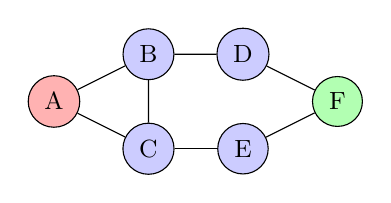
\begin{tikzpicture}[scale=0.6, every node/.style={font=\small}]
            \node[circle, draw, fill=red!30] (A) at (0,2) {A};
            \node[circle, draw, fill=blue!20] (B) at (2,3) {B};
            \node[circle, draw, fill=blue!20] (C) at (2,1) {C};
            \node[circle, draw, fill=blue!20] (D) at (4,3) {D};
            \node[circle, draw, fill=blue!20] (E) at (4,1) {E};
            \node[circle, draw, fill=green!30] (F) at (6,2) {F};
            
            \draw (A) -- (B);
            \draw (A) -- (C);
            \draw (B) -- (D);
            \draw (B) -- (C);
            \draw (C) -- (E);
            \draw (D) -- (F);
            \draw (E) -- (F);
        \end{tikzpicture}
        \end{center}
        
        \column{0.55\textwidth}
        \textbf{Routing Table at Node A:}
        \begin{center}
        \begin{tabular}{|c|c|}
            \hline
            \textbf{Destination} & \textbf{Next Hop} \\
            \hline
            B & B \\
            C & C \\
            D & B \\
            E & C \\
            F & B or C \\
            \hline
        \end{tabular}
        \end{center}
    \end{columns}
    
    \vspace{0.3cm}
    \begin{alertblock}{Packet Forwarding}
        Router checks destination in table $\rightarrow$ forwards to next hop $\rightarrow$ process repeats until destination reached.
    \end{alertblock}
\end{frame}

\begin{frame}{Shortest Path Problem}
    \textbf{Objective:} Compute optimal paths between any two nodes given complete network topology.
    
    \vspace{0.3cm}
    \begin{columns}
        \column{0.5\textwidth}
        \textbf{Graph Representation:}
        \begin{itemize}
            \item Nodes $\rightarrow$ routers/devices
            \item Edges $\rightarrow$ links
            \item Edge weights $\rightarrow$ ``distance'' metric
        \end{itemize}
        
        \vspace{0.3cm}
        \textbf{Possible Metrics:}
        \begin{itemize}
            \item Hop count (simplest)
            \item Propagation delay
            \item Link capacity/bandwidth
            \item Energy remaining at nodes
            \item Expected Transmission Count (ETX)
        \end{itemize}
        
        \column{0.5\textwidth}
        \begin{center}
        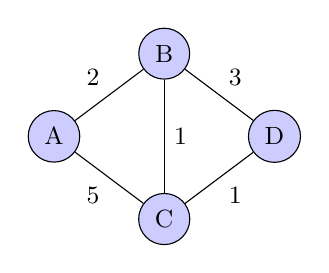
\begin{tikzpicture}[scale=0.7, every node/.style={font=\small}]
            \node[circle, draw, fill=blue!20] (A) at (0,2) {A};
            \node[circle, draw, fill=blue!20] (B) at (2,3.5) {B};
            \node[circle, draw, fill=blue!20] (C) at (2,0.5) {C};
            \node[circle, draw, fill=blue!20] (D) at (4,2) {D};
            
            \draw (A) -- node[above left] {2} (B);
            \draw (A) -- node[below left] {5} (C);
            \draw (B) -- node[above right] {3} (D);
            \draw (C) -- node[below right] {1} (D);
            \draw (B) -- node[right] {1} (C);
        \end{tikzpicture}
        \end{center}
        
        \textbf{A $\rightarrow$ D:}
        \begin{itemize}
            \item A-B-D: cost = 5
            \item A-C-D: cost = 6
            \item A-B-C-D: cost = 4 $\checkmark$
        \end{itemize}
    \end{columns}
\end{frame}

\begin{frame}{Dijkstra's Algorithm}
    \textbf{Published 1959 by Edsger Dijkstra}
    
    \vspace{0.3cm}
    \begin{columns}
        \column{0.55\textwidth}
        \textbf{Algorithm:}
        \begin{enumerate}
            \item Mark all nodes unvisited, set distance to $\infty$
            \item Set source distance to 0
            \item For current node, update neighbor distances
            \item Mark current node visited
            \item Select unvisited node with smallest distance
            \item Repeat until destination reached
        \end{enumerate}
        
        \column{0.45\textwidth}
        \begin{alertblock}{Requirement}
            Requires \textbf{complete knowledge} of network topology!
        \end{alertblock}
        
        \vspace{0.3cm}
        \textbf{When feasible:}
        \begin{itemize}
            \item Fixed networks with static links
            \item Centralized controller
        \end{itemize}
        
        \textbf{When NOT feasible:}
        \begin{itemize}
            \item Dynamic traffic loads
            \item Mobile/sleeping nodes
            \item Large-scale IoT deployments
        \end{itemize}
    \end{columns}
\end{frame}

\begin{frame}{Flooding}
    \textbf{Simple approach:} Send every received packet through \textbf{all links} except the incoming one.
    
    \vspace{0.3cm}
    \textbf{Problem:} Generates exponential duplicates $\rightarrow$ must be controlled!
    
    \vspace{0.3cm}
    \begin{columns}
        \column{0.5\textwidth}
        \begin{block}{Option 1: Hop Counter (TTL)}
            \begin{itemize}
                \item Add counter in header
                \item Decrement at each hop
                \item Discard when counter = 0
                \item Initial value = network diameter
            \end{itemize}
            \textit{Still exponential duplicates!}
        \end{block}
        
        \column{0.5\textwidth}
        \begin{block}{Option 2: Sequence Number}
            \begin{itemize}
                \item Track (source, seq\#) pairs
                \item Discard if already seen
                \item Memory grows unbounded
                \item Store only max seq\# per source
            \end{itemize}
            \textit{What about out-of-order?}
        \end{block}
    \end{columns}
\end{frame}

\begin{frame}{Flooding: When It's Useful}
    \textbf{Despite inefficiency, controlled flooding has advantages:}
    
    \vspace{0.5cm}
    \begin{columns}
        \column{0.5\textwidth}
        \begin{exampleblock}{Use Cases}
            \begin{itemize}
                \item \textbf{Broadcasting} control information
                \item \textbf{Route discovery} in reactive protocols
                \item \textbf{Military/emergency} networks (robustness)
                \item \textbf{Benchmark} for other protocols
            \end{itemize}
        \end{exampleblock}
        
        \column{0.5\textwidth}
        \begin{alertblock}{Key Property}
            If \textbf{any path exists} between source and destination, flooding will find it.
            
            \vspace{0.2cm}
            Explores all paths in parallel $\rightarrow$ finds shortest delay (ignoring congestion).
        \end{alertblock}
    \end{columns}
    
    \vspace{0.5cm}
    \textbf{IoT Application:} Many IoT protocols use controlled flooding for initial route discovery (AODV, RPL).
\end{frame}

\begin{frame}{Distance Vector Routing (DVR)}
    \textbf{Each router maintains a distance vector:} best distance to each destination + next hop.
    
    \vspace{0.3cm}
    \begin{columns}
        \column{0.55\textwidth}
        \textbf{Bellman-Ford Algorithm (1957/1962):}
        \begin{enumerate}
            \item Initialize: distance to self = 0, others = $\infty$
            \item Exchange vectors with neighbors
            \item Update: $D(v) = \min_w[c(u,w) + D_w(v)]$
            \item Repeat until convergence
        \end{enumerate}
        
        \vspace{0.3cm}
        \textbf{Used in:}
        \begin{itemize}
            \item Original ARPANET
            \item RIP (Routing Information Protocol)
        \end{itemize}
        
        \column{0.45\textwidth}
        \begin{alertblock}{Count-to-Infinity Problem}
            If a link fails, bad news travels slowly.
            
            \vspace{0.2cm}
            Node A thinks it can reach X via B.
            Node B thinks it can reach X via A.
            Distance increments slowly to $\infty$.
        \end{alertblock}
    \end{columns}
\end{frame}

\begin{frame}{Link State Routing (LSR)}
    \textbf{Replaced DVR in ARPANET (1979)} -- much faster convergence!
    
    \vspace{0.3cm}
    \textbf{Basic Idea:} Each router:
    \begin{enumerate}
        \item \textbf{Discover} neighbors and their addresses
        \item \textbf{Measure} cost/distance to each neighbor
        \item \textbf{Construct} Link State Packet (LSP) with this info
        \item \textbf{Flood} LSP to all other routers
        \item \textbf{Compute} shortest paths using Dijkstra
    \end{enumerate}
    
    \vspace{0.3cm}
    \begin{columns}
        \column{0.5\textwidth}
        \begin{exampleblock}{Advantages}
            \begin{itemize}
                \item Fast convergence
                \item Each router has full topology
                \item Used in OSPF, IS-IS
            \end{itemize}
        \end{exampleblock}
        
        \column{0.5\textwidth}
        \begin{alertblock}{Disadvantages}
            \begin{itemize}
                \item Higher memory requirements
                \item More complex implementation
                \item Flooding overhead for LSPs
            \end{itemize}
        \end{alertblock}
    \end{columns}
\end{frame}

\begin{frame}{DVR vs LSR: Scalability Issues}
    \textbf{As networks grow, routing tables grow proportionally:}
    
    \vspace{0.3cm}
    \begin{itemize}
        \item More \textbf{memory} consumed at each router
        \item More \textbf{CPU time} to scan tables
        \item More \textbf{bandwidth} for status updates
    \end{itemize}
    
    \vspace{0.3cm}
    \begin{alertblock}{Fundamental Limit}
        At some scale, it's \textbf{no longer feasible} for every router to have an entry for every other router!
    \end{alertblock}
    
    \vspace{0.3cm}
    \textbf{Solution: Hierarchical Routing}
    \begin{itemize}
        \item Routers divided into \textbf{regions}
        \item Full knowledge within region, summary for other regions
        \item Multi-level: regions $\rightarrow$ clusters $\rightarrow$ zones $\rightarrow$ groups
        \item Example: telephone network, Internet AS structure
    \end{itemize}
\end{frame}

%==============================================================================
\section{Broadcast, Multicast, and Anycast}
%==============================================================================

\begin{frame}{Broadcast Routing}
    \textbf{Broadcasting:} Sending a packet to \textbf{all} destinations simultaneously.
    
    \vspace{0.3cm}
    \textbf{Applications:} Weather alerts, traffic updates, live radio, network discovery.
    
    \vspace{0.3cm}
    \begin{columns}
        \column{0.5\textwidth}
        \textbf{Methods (worst to best):}
        \begin{enumerate}
            \item \textbf{N unicasts:} Send distinct packet to each destination -- very inefficient
            \item \textbf{Multi-destination:} Packet carries destination list -- still inefficient
            \item \textbf{Flooding:} Simple but generates duplicates
            \item \textbf{Spanning tree:} Optimal but requires tree construction
        \end{enumerate}
        
        \column{0.5\textwidth}
        \begin{exampleblock}{Wireless Advantage}
            In wireless, broadcasting to $n$ neighbors can cost:
            \begin{itemize}
                \item Same as 1 unicast (if RX costs ignored)
                \item 1 TX + $n$ RX (if synchronized)
                \item $n$ unicasts (no multicast support)
            \end{itemize}
            
            \textbf{Wireless multicast advantage} when local multicast $<$ repeated unicasts.
        \end{exampleblock}
    \end{columns}
\end{frame}

\begin{frame}{Multicast and Anycast}
    \begin{columns}
        \column{0.5\textwidth}
        \begin{block}{Multicast}
            Send to a \textbf{well-defined group} (large but $\ll$ total network).
            
            \vspace{0.2cm}
            \textbf{Examples:}
            \begin{itemize}
                \item Multi-player gaming
                \item Live video streaming
                \item Sensor group updates
            \end{itemize}
            
            \vspace{0.2cm}
            Requires group membership management.
        \end{block}
        
        \column{0.5\textwidth}
        \begin{block}{Anycast}
            Deliver to the \textbf{nearest member} of a group.
            
            \vspace{0.2cm}
            \textbf{Examples:}
            \begin{itemize}
                \item DNS root servers
                \item CDN edge servers
                \item \textbf{WSN data collection!}
            \end{itemize}
            
            \vspace{0.2cm}
            All group members share same address. DVR/LSR naturally finds closest.
        \end{block}
    \end{columns}
    
    \vspace{0.3cm}
    \begin{alertblock}{IoT Relevance}
        In sensor networks, anycast is natural: ``send reading to \textbf{any} gateway'' -- we care about the data, not which gateway receives it.
    \end{alertblock}
\end{frame}

%==============================================================================
\section{Mobile and Ad-Hoc Routing}
%==============================================================================

\begin{frame}{Mobile Routing Challenges}
    \textbf{Mobile nodes introduce several challenges:}
    
    \vspace{0.3cm}
    \begin{columns}
        \column{0.5\textwidth}
        \textbf{Scenario A: Mobile Hosts, Static Routers}
        \begin{itemize}
            \item Host moves between networks
            \item \textbf{Option 1:} Get new address at each location (simple, requires reconnection)
            \item \textbf{Option 2:} Keep same address (Mobile IP, home agent forwarding)
        \end{itemize}
        
        \column{0.5\textwidth}
        \textbf{Scenario B: Mobile Ad-Hoc Networks (MANETs)}
        \begin{itemize}
            \item Both hosts AND routers are mobile
            \item Nodes appear/disappear dynamically
            \item Topology constantly changing
            \item \textbf{Every node is a potential router}
        \end{itemize}
    \end{columns}
    
    \vspace{0.3cm}
    \begin{exampleblock}{MANET Applications}
        Military battlefield networks, disaster recovery, vehicular networks, mobile sensor networks.
    \end{exampleblock}
\end{frame}

\begin{frame}{Ad-Hoc Routing Classification}
    \textbf{1. When does the protocol operate?}
    
    \vspace{0.3cm}
    \begin{columns}
        \column{0.33\textwidth}
        \begin{block}{Proactive}
            \begin{itemize}
                \item Routes always up-to-date
                \item Table-driven
                \item Low latency for data
                \item High control overhead
            \end{itemize}
            \textit{Example: OLSR}
        \end{block}
        
        \column{0.33\textwidth}
        \begin{block}{Reactive}
            \begin{itemize}
                \item Routes on-demand
                \item Low idle overhead
                \item Higher initial latency
                \item Good for sparse traffic
            \end{itemize}
            \textit{Example: AODV}
        \end{block}
        
        \column{0.33\textwidth}
        \begin{block}{Hybrid}
            \begin{itemize}
                \item Combines both approaches
                \item Proactive within zone
                \item Reactive across zones
            \end{itemize}
            \textit{Example: ZRP}
        \end{block}
    \end{columns}
    
    \vspace{0.3cm}
    \textbf{2. Other classifications:}
    \begin{itemize}
        \item \textbf{Topology:} Flat vs Hierarchical
        \item \textbf{Addressing:} Arbitrary ID vs Geographic position vs Structured
    \end{itemize}
\end{frame}

\begin{frame}{AODV: Ad-hoc On-demand Distance Vector}
    \textbf{Reactive protocol:} Routes discovered only when needed.
    
    \vspace{0.3cm}
    \textbf{Route Discovery Process:}
    \begin{enumerate}
        \item Source checks routing table for valid route
        \item If no route, broadcast \textbf{Route Request (RREQ)} using controlled flooding
        \item Intermediate nodes record \textbf{reverse path} (back to source)
        \item Destination sends \textbf{Route Reply (RREP)} along reverse path
        \item Each node learns next hop toward destination
    \end{enumerate}
    
    \vspace{0.3cm}
    \begin{columns}
        \column{0.5\textwidth}
        \begin{exampleblock}{Optimization: Expanding Ring}
            Start with TTL=1, increment if no reply. Reduces flooding for nearby destinations.
        \end{exampleblock}
        
        \column{0.5\textwidth}
        \begin{alertblock}{Sequence Numbers}
            Destination controls seq\# to ensure fresh routes. Higher seq\# = more recent route.
        \end{alertblock}
    \end{columns}
\end{frame}

\begin{frame}{AODV: Route Discovery Visualization}
    \begin{center}
    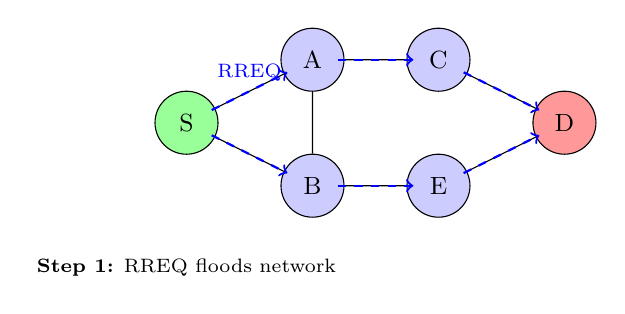
\begin{tikzpicture}[scale=0.8, every node/.style={font=\small}]
        % Nodes
        \node[circle, draw, fill=green!40, minimum size=0.8cm] (S) at (0,2) {S};
        \node[circle, draw, fill=blue!20, minimum size=0.8cm] (A) at (2,3) {A};
        \node[circle, draw, fill=blue!20, minimum size=0.8cm] (B) at (2,1) {B};
        \node[circle, draw, fill=blue!20, minimum size=0.8cm] (C) at (4,3) {C};
        \node[circle, draw, fill=blue!20, minimum size=0.8cm] (E) at (4,1) {E};
        \node[circle, draw, fill=red!40, minimum size=0.8cm] (D) at (6,2) {D};
        
        % Links
        \draw (S) -- (A);
        \draw (S) -- (B);
        \draw (A) -- (C);
        \draw (A) -- (B);
        \draw (B) -- (E);
        \draw (C) -- (D);
        \draw (E) -- (D);
        
        % RREQ arrows (broadcast)
        \draw[->, thick, blue, dashed] (0.4,2.2) -- (1.6,2.8);
        \draw[->, thick, blue, dashed] (0.4,1.8) -- (1.6,1.2);
        \draw[->, thick, blue, dashed] (2.4,3) -- (3.6,3);
        \draw[->, thick, blue, dashed] (2.4,1) -- (3.6,1);
        \draw[->, thick, blue, dashed] (4.4,2.8) -- (5.6,2.2);
        \draw[->, thick, blue, dashed] (4.4,1.2) -- (5.6,1.8);
        
        % Labels
        \node[blue, font=\scriptsize] at (1,2.8) {RREQ};
        \node[font=\scriptsize] at (0,-0.3) {\textbf{Step 1:} RREQ floods network};
    \end{tikzpicture}
    \hspace{1cm}
    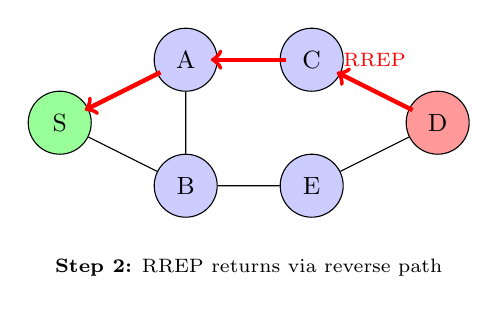
\begin{tikzpicture}[scale=0.8, every node/.style={font=\small}]
        % Nodes (same layout)
        \node[circle, draw, fill=green!40, minimum size=0.8cm] (S) at (0,2) {S};
        \node[circle, draw, fill=blue!20, minimum size=0.8cm] (A) at (2,3) {A};
        \node[circle, draw, fill=blue!20, minimum size=0.8cm] (B) at (2,1) {B};
        \node[circle, draw, fill=blue!20, minimum size=0.8cm] (C) at (4,3) {C};
        \node[circle, draw, fill=blue!20, minimum size=0.8cm] (E) at (4,1) {E};
        \node[circle, draw, fill=red!40, minimum size=0.8cm] (D) at (6,2) {D};
        
        % Links
        \draw (S) -- (A);
        \draw (S) -- (B);
        \draw (A) -- (C);
        \draw (A) -- (B);
        \draw (B) -- (E);
        \draw (C) -- (D);
        \draw (E) -- (D);
        
        % RREP arrows (unicast back)
        \draw[->, ultra thick, red] (5.6,2.2) -- (4.4,2.8);
        \draw[->, ultra thick, red] (3.6,3) -- (2.4,3);
        \draw[->, ultra thick, red] (1.6,2.8) -- (0.4,2.2);
        
        % Labels
        \node[red, font=\scriptsize] at (5,3) {RREP};
        \node[font=\scriptsize] at (3,-0.3) {\textbf{Step 2:} RREP returns via reverse path};
    \end{tikzpicture}
    \end{center}
\end{frame}

\begin{frame}{AODV: Route Maintenance}
    \textbf{Network topology can change:} nodes move, fail, or run out of battery.
    
    \vspace{0.3cm}
    \textbf{Maintenance Mechanism:}
    \begin{enumerate}
        \item Nodes periodically broadcast \textbf{Hello messages}
        \item If neighbor doesn't reply $\rightarrow$ assume link broken
        \item Purge routes through that neighbor
        \item Send \textbf{Route Error (RERR)} to affected sources
        \item Sources initiate new route discovery
    \end{enumerate}
    
    \vspace{0.3cm}
    \begin{columns}
        \column{0.5\textwidth}
        \begin{exampleblock}{Local Repair}
            Intermediate nodes can attempt local route discovery before notifying source.
        \end{exampleblock}
        
        \column{0.5\textwidth}
        \begin{alertblock}{Energy Implication}
            Hello messages consume energy even when no data flows. Trade-off: detection speed vs energy.
        \end{alertblock}
    \end{columns}
\end{frame}

\begin{frame}{OLSR: Optimized Link State Routing}
    \textbf{Proactive protocol:} Routes maintained continuously.
    
    \vspace{0.3cm}
    \textbf{Key Optimization: Multipoint Relays (MPRs)}
    \begin{itemize}
        \item Each node selects a subset of neighbors as MPRs
        \item Only MPRs forward control messages
        \item Reduces flooding overhead significantly
    \end{itemize}
    
    \vspace{0.3cm}
    \begin{columns}
        \column{0.5\textwidth}
        \textbf{Messages:}
        \begin{itemize}
            \item \textbf{Hello:} Neighbor discovery, MPR selection
            \item \textbf{TC (Topology Control):} Advertise MPR selectors
        \end{itemize}
        
        \column{0.5\textwidth}
        \textbf{Comparison with AODV:}
        \begin{itemize}
            \item Lower latency (routes ready)
            \item Higher control overhead
            \item Better for frequent communication
        \end{itemize}
    \end{columns}
    
    \vspace{0.3cm}
    \begin{alertblock}{When to Use}
        \textbf{OLSR:} Dense networks, frequent traffic. \textbf{AODV:} Sparse traffic, energy-constrained nodes.
    \end{alertblock}
\end{frame}

%==============================================================================
\section{IoT Routing: RPL}
%==============================================================================

\begin{frame}{Routing Requirements for IoT}
    \textbf{IoT networks have unique characteristics:}
    
    \vspace{0.3cm}
    \begin{columns}
        \column{0.5\textwidth}
        \begin{itemize}
            \item \textbf{Energy} is the primary constraint
            \item \textbf{Limited processing} power
            \item \textbf{Very dynamic} topologies
            \item Link failures (wireless)
            \item Node failures (low-cost hardware)
            \item Node mobility (some scenarios)
        \end{itemize}
        
        \column{0.5\textwidth}
        \begin{itemize}
            \item \textbf{Large scale} deployments
            \item \textbf{Self-managed} (auto-discovery)
            \item \textbf{Harsh environments}
            \item Asymmetric links common
            \item Data aggregation needed
            \item Multiple traffic patterns
        \end{itemize}
    \end{columns}
    
    \vspace{0.3cm}
    \begin{alertblock}{Traditional Protocols Fall Short}
        AODV/OLSR designed for MANETs with laptops -- not optimized for constrained, lossy IoT networks.
    \end{alertblock}
\end{frame}

\begin{frame}{RPL: Routing Protocol for LLNs}
    \textbf{IETF RFC 6550 (March 2012)} -- ``Ripple''
    
    \vspace{0.3cm}
    \textbf{Designed for Low-Power and Lossy Networks (LLNs)}
    
    \vspace{0.3cm}
    \begin{columns}
        \column{0.5\textwidth}
        \textbf{Key Features:}
        \begin{itemize}
            \item \textbf{Proactive} distance-vector routing
            \item \textbf{Source routing} support
            \item Link-layer agnostic
            \item Optimized for constrained devices
        \end{itemize}
        
        \column{0.5\textwidth}
        \textbf{Traffic Patterns Supported:}
        \begin{itemize}
            \item \textbf{MP2P:} Many-to-one (sensors $\rightarrow$ gateway)
            \item \textbf{P2MP:} One-to-many (gateway $\rightarrow$ sensors)
            \item \textbf{P2P:} Device-to-device
        \end{itemize}
    \end{columns}
    
    \vspace{0.3cm}
    \begin{exampleblock}{Primary Use Case}
        Sensor networks reporting to a central collection point (DODAG root).
    \end{exampleblock}
\end{frame}

\begin{frame}{RPL: DODAG Construction}
    \textbf{DODAG = Destination-Oriented Directed Acyclic Graph}
    
    \vspace{0.3cm}
    \begin{columns}
        \column{0.5\textwidth}
        \begin{center}
        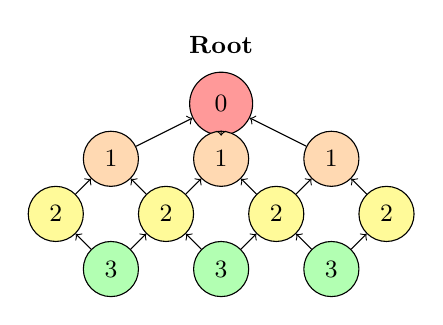
\begin{tikzpicture}[scale=0.7, every node/.style={font=\small}]
            % Root
            \node[circle, draw, fill=red!40, minimum size=0.8cm] (R) at (3,4) {0};
            \node[above=0.1cm of R] {\textbf{Root}};
            
            % Rank 1
            \node[circle, draw, fill=orange!30, minimum size=0.7cm] (A) at (1,3) {1};
            \node[circle, draw, fill=orange!30, minimum size=0.7cm] (B) at (3,3) {1};
            \node[circle, draw, fill=orange!30, minimum size=0.7cm] (C) at (5,3) {1};
            
            % Rank 2
            \node[circle, draw, fill=yellow!40, minimum size=0.7cm] (D) at (0,2) {2};
            \node[circle, draw, fill=yellow!40, minimum size=0.7cm] (E) at (2,2) {2};
            \node[circle, draw, fill=yellow!40, minimum size=0.7cm] (F) at (4,2) {2};
            \node[circle, draw, fill=yellow!40, minimum size=0.7cm] (G) at (6,2) {2};
            
            % Rank 3
            \node[circle, draw, fill=green!30, minimum size=0.7cm] (H) at (1,1) {3};
            \node[circle, draw, fill=green!30, minimum size=0.7cm] (I) at (3,1) {3};
            \node[circle, draw, fill=green!30, minimum size=0.7cm] (J) at (5,1) {3};
            
            % Edges (upward)
            \draw[->] (A) -- (R);
            \draw[->] (B) -- (R);
            \draw[->] (C) -- (R);
            \draw[->] (D) -- (A);
            \draw[->] (E) -- (A);
            \draw[->] (E) -- (B);
            \draw[->] (F) -- (B);
            \draw[->] (F) -- (C);
            \draw[->] (G) -- (C);
            \draw[->] (H) -- (D);
            \draw[->] (H) -- (E);
            \draw[->] (I) -- (E);
            \draw[->] (I) -- (F);
            \draw[->] (J) -- (F);
            \draw[->] (J) -- (G);
        \end{tikzpicture}
        \end{center}
        
        \column{0.5\textwidth}
        \textbf{Rank:} Distance from root (not hops!)
        
        \vspace{0.2cm}
        \textbf{Control Messages:}
        \begin{itemize}
            \item \textbf{DIO} (DODAG Info Object): Broadcast to build tree
            \item \textbf{DIS} (DODAG Info Solicitation): Request DIO
            \item \textbf{DAO} (Destination Advertisement): Downward routes
        \end{itemize}
        
        \vspace{0.2cm}
        \textbf{Objective Function:}
        \begin{itemize}
            \item Defines how rank is computed
            \item Can optimize for hops, ETX, energy...
        \end{itemize}
    \end{columns}
\end{frame}

\begin{frame}{RPL: Objective Functions}
    \textbf{The Objective Function (OF) determines path selection criteria.}
    
    \vspace{0.3cm}
    \begin{columns}
        \column{0.5\textwidth}
        \begin{block}{OF0 (RFC 6552)}
            \begin{itemize}
                \item Simple hop count
                \item Rank = parent rank + increment
                \item Low overhead
                \item May choose poor links
            \end{itemize}
        \end{block}
        
        \column{0.5\textwidth}
        \begin{block}{MRHOF (RFC 6719)}
            \begin{itemize}
                \item Minimum Rank with Hysteresis
                \item Uses ETX (Expected TX Count)
                \item Prefers reliable links
                \item Hysteresis prevents flapping
            \end{itemize}
        \end{block}
    \end{columns}
    
    \vspace{0.3cm}
    \begin{exampleblock}{ETX Calculation}
        $\text{ETX} = \frac{1}{P_{forward} \times P_{reverse}}$
        
        \vspace{0.2cm}
        If forward delivery = 90\%, reverse ACK = 80\%: ETX = $\frac{1}{0.9 \times 0.8} = 1.39$
    \end{exampleblock}
\end{frame}

%==============================================================================
\section{IPv6 for IoT}
%==============================================================================

\begin{frame}{Why IP for IoT?}
    \textbf{Benefits of IP-based IoT:}
    
    \vspace{0.3cm}
    \begin{columns}
        \column{0.5\textwidth}
        \begin{itemize}
            \item \textbf{Interoperability:} End-to-end with any IP device
            \item \textbf{Established security:} Authentication, firewalls
            \item \textbf{Naming/addressing:} DNS, DHCP
            \item \textbf{Proxy architectures:} NAT, load balancing, caching
        \end{itemize}
        
        \column{0.5\textwidth}
        \begin{itemize}
            \item \textbf{Application protocols:} HTTP, CoAP, MQTT
            \item \textbf{Management tools:} ping, traceroute
            \item \textbf{Transport options:} TCP, UDP
            \item \textbf{Industry adoption:} Most standards support IP
        \end{itemize}
    \end{columns}
    
    \vspace{0.3cm}
    \begin{alertblock}{Design Philosophy}
        Instead of proprietary gateways translating between IoT protocols and IP, make IoT devices \textbf{native IP speakers}.
    \end{alertblock}
\end{frame}

\begin{frame}{IPv4 vs IPv6 for IoT}
    \begin{columns}
        \column{0.5\textwidth}
        \begin{block}{IPv4 Limitations}
            \begin{itemize}
                \item 32-bit addresses ($\sim$4 billion)
                \item Address exhaustion
                \item NAT required for IoT scale
                \item NAT breaks end-to-end
                \item Complex header (13 fields)
            \end{itemize}
        \end{block}
        
        \column{0.5\textwidth}
        \begin{block}{IPv6 Advantages}
            \begin{itemize}
                \item 128-bit addresses ($3.4 \times 10^{38}$)
                \item No NAT needed
                \item Simpler header (7 fields)
                \item Built-in security (IPSec)
                \item Better QoS support
            \end{itemize}
        \end{block}
    \end{columns}
    
    \vspace{0.3cm}
    \begin{exampleblock}{Scale Comparison}
        \textbf{IPv4:} $\sim$4 billion addresses (less than 1 per person)
        
        \textbf{IPv6:} $\sim 10^{38}$ addresses ($\sim 10^{28}$ per person on Earth!)
    \end{exampleblock}
\end{frame}

\begin{frame}{IPv6 Header Structure}
    \begin{center}
    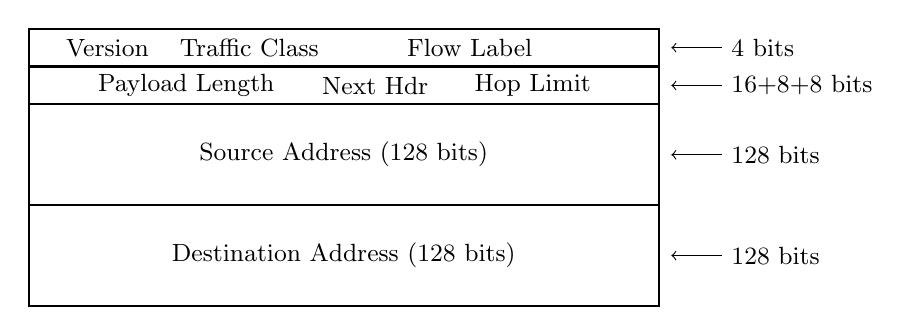
\begin{tikzpicture}[scale=0.8, every node/.style={font=\small}]
        \draw[thick] (0,0) rectangle (10,0.6);
        \node at (1.25,0.3) {Version};
        \node at (3.5,0.3) {Traffic Class};
        \node at (7,0.3) {Flow Label};
        
        \draw[thick] (0,-0.6) rectangle (10,0);
        \node at (2.5,-0.3) {Payload Length};
        \node at (5.5,-0.3) {Next Hdr};
        \node at (8,-0.3) {Hop Limit};
        
        \draw[thick] (0,-2.2) rectangle (10,-0.6);
        \node at (5,-1.4) {Source Address (128 bits)};
        
        \draw[thick] (0,-3.8) rectangle (10,-2.2);
        \node at (5,-3) {Destination Address (128 bits)};
        
        % Annotations
        \draw[<-] (10.2,0.3) -- (11,0.3) node[right] {4 bits};
        \draw[<-] (10.2,-0.3) -- (11,-0.3) node[right] {16+8+8 bits};
        \draw[<-] (10.2,-1.4) -- (11,-1.4) node[right] {128 bits};
        \draw[<-] (10.2,-3) -- (11,-3) node[right] {128 bits};
    \end{tikzpicture}
    \end{center}
    
    \vspace{0.3cm}
    \textbf{Fixed 40-byte header} (vs variable IPv4 header up to 60 bytes)
    
    \vspace{0.2cm}
    \begin{itemize}
        \item \textbf{No checksum:} Link layer + transport layer handle this
        \item \textbf{No fragmentation fields:} Handled by extension headers
        \item \textbf{Flow Label:} Enables QoS without deep packet inspection
    \end{itemize}
\end{frame}

\begin{frame}{6LoWPAN: IPv6 over Low-Power WPANs}
    \textbf{Problem:} IPv6 header (40 bytes) + UDP (8 bytes) won't fit in IEEE 802.15.4 frame (127 bytes max)!
    
    \vspace{0.3cm}
    \textbf{6LoWPAN Solution (RFC 4944, 6282):}
    \begin{itemize}
        \item \textbf{Header compression:} 40-byte IPv6 $\rightarrow$ 2-3 bytes typical
        \item \textbf{Fragmentation:} Large packets split across frames
        \item \textbf{Mesh addressing:} Multi-hop at link layer
    \end{itemize}
    
    \vspace{0.3cm}
    \begin{columns}
        \column{0.5\textwidth}
        \begin{exampleblock}{Compression Techniques}
            \begin{itemize}
                \item Omit fields derivable from L2
                \item Use link-local prefix (known)
                \item Elide addresses from 802.15.4
                \item Context-based compression
            \end{itemize}
        \end{exampleblock}
        
        \column{0.5\textwidth}
        \begin{alertblock}{After Compression}
            IPv6 (40B) + UDP (8B) = 48 bytes
            
            $\downarrow$ 6LoWPAN compression
            
            IPHC (2-3B) + UDP (4B) = 6-7 bytes
            
            \textbf{85\% reduction!}
        \end{alertblock}
    \end{columns}
\end{frame}

%==============================================================================
\section{Summary}
%==============================================================================

\begin{frame}{Module Summary}
    \textbf{Network Layer enables end-to-end communication across multiple hops.}
    
    \vspace{0.3cm}
    \begin{columns}
        \column{0.5\textwidth}
        \textbf{Routing Fundamentals:}
        \begin{itemize}
            \item DVR: Simple, count-to-infinity problem
            \item LSR: Faster convergence, more overhead
            \item Hierarchical: Scalability solution
        \end{itemize}
        
        \vspace{0.2cm}
        \textbf{Ad-Hoc Routing:}
        \begin{itemize}
            \item AODV: Reactive, on-demand
            \item OLSR: Proactive, MPR optimization
        \end{itemize}
        
        \column{0.5\textwidth}
        \textbf{IoT-Specific:}
        \begin{itemize}
            \item RPL: Designed for LLNs
            \item DODAG tree structure
            \item Objective functions (OF0, MRHOF)
        \end{itemize}
        
        \vspace{0.2cm}
        \textbf{IPv6 for IoT:}
        \begin{itemize}
            \item Massive address space
            \item 6LoWPAN header compression
            \item End-to-end IP connectivity
        \end{itemize}
    \end{columns}
    
    \vspace{0.3cm}
    \begin{alertblock}{Design Trade-off}
        \textbf{Routing overhead} vs \textbf{route freshness} vs \textbf{energy consumption}
    \end{alertblock}
\end{frame}

\begin{frame}{Questions?}
    \begin{center}
        \Huge Questions?
        
        \vspace{1cm}
        \normalsize
        \textbf{Eduardo Baena}\\
        \texttt{e.baena@northeastern.edu}
        
        \vspace{0.5cm}
        \textit{EECE5155: Wireless Sensor Networks and the Internet of Things}\\
        Spring 2026
    \end{center}
\end{frame}

\end{document}
